\documentclass[border=3pt]{standalone}
% Preâmbulo compartilhado pelos diagramas TikZ da aula
\usepackage[T1]{fontenc}
\usepackage[utf8]{inputenc}
\usepackage{lmodern}
\usepackage{amsmath}
\usepackage{xcolor}
\usepackage{tikz}
\usetikzlibrary{arrows.meta,angles,quotes,decorations.pathmorphing,calc,
                positioning,shapes.geometric,backgrounds,fit}

% Paleta (mesma dos SVGs originais)
\definecolor{dblue}{HTML}{2A5B8C}
\definecolor{dorange}{HTML}{B3541E}
\definecolor{dgreen}{HTML}{4A7C59}
\definecolor{dred}{HTML}{9C4B4B}
\definecolor{dcream}{HTML}{F4F1EA}
\definecolor{dshade}{HTML}{DDD7C9}

% Estilos comuns (prefixo d... para não colidir com chaves internas do pgf)
\tikzset{
  >={Stealth[length=2mm]},
  dguide/.style={gray!55, dashed, line width=0.4pt},
  daxis/.style={gray!60, line width=0.7pt, ->},
  dbody/.style={fill=black!3, draw=black!80, line width=1pt},
  dacc/.style={draw=dblue, line width=1pt},
  dlbl/.style={black!55, font=\small},
  dsub/.style={black!45, font=\footnotesize},
  dstate/.style={circle, draw=black!80, fill=dcream, line width=1pt,
                 minimum size=17mm, font=\large, inner sep=1pt},
  dobs/.style={circle, draw=black!80, fill=dshade, line width=1pt,
               minimum size=14mm, font=\large, inner sep=1pt},
  dbox/.style={rounded corners=2pt, draw=black!80, fill=dcream, line width=1pt,
               align=center, inner sep=6pt},
  dtrans/.style={->, dblue, line width=1pt},
  dmeas/.style={->, dorange, line width=1pt},
}

\begin{document}
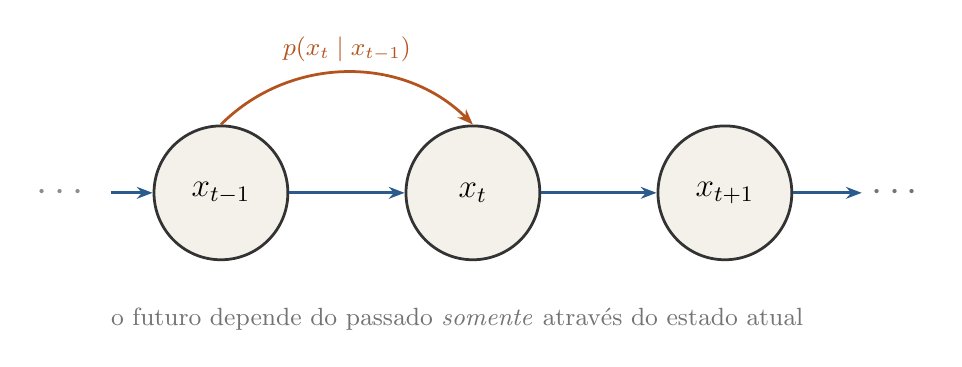
\begin{tikzpicture}[x=1cm,y=1cm]

  \node[dstate] (a) at (0,0)   {$x_{t-1}$};
  \node[dstate] (b) at (3.2,0) {$x_t$};
  \node[dstate] (c) at (6.4,0) {$x_{t+1}$};
  \node[black!55, font=\Large] (d) at (8.6,0) {$\cdots$};
  \node[black!45, font=\Large] at (-2.0,0) {$\cdots$};

  \draw[dtrans, line width=1.1pt] (-1.4,0) -- (a);
  \draw[dtrans, line width=1.1pt] (a) -- (b);
  \draw[dtrans, line width=1.1pt] (b) -- (c);
  \draw[dtrans, line width=1.1pt] (c) -- (d);

  % destaque de dependência
  \draw[dorange, line width=1pt, ->, bend left=45]
       (a.north) to node[above, dorange, font=\small] {$p(x_t\mid x_{t-1})$} (b.north);

  \node[dlbl] at (3.0,-1.6)
    {o futuro depende do passado \emph{somente} através do estado atual};

\end{tikzpicture}
\end{document}
